% C086 accurate diagram: H:x²/4-y²/12=1; F1=(-4,0), F2=(4,0), P=(3,sqrt(15)).
% Lengths PF1=8, PF2=4, F1F2=8; lambda=2, e=2 (<3).
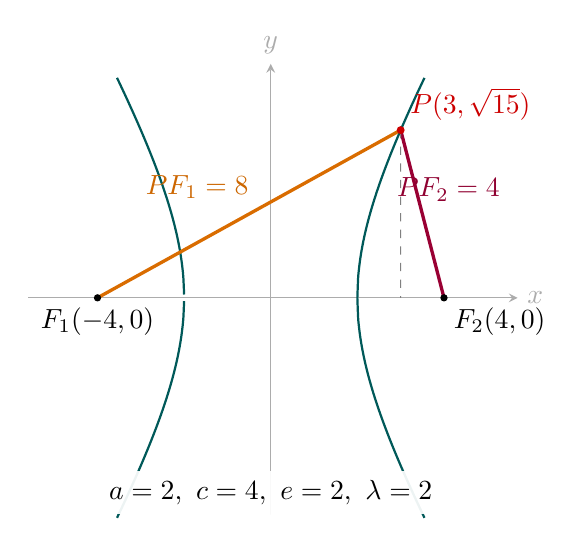
\begin{tikzpicture}[scale=0.55,>=stealth]
  \draw[->,gray!65] (-5.6,0)--(5.7,0) node[right] {$x$};
  \draw[->,gray!65] (0,-5.0)--(0,5.4) node[above] {$y$};
  \draw[teal!70!black,thick,samples=90,domain=2:3.55,smooth]
    plot (\x,{sqrt(3*(\x*\x-4))});
  \draw[teal!70!black,thick,samples=90,domain=2:3.55,smooth]
    plot (\x,{-sqrt(3*(\x*\x-4))});
  \draw[teal!70!black,thick,samples=90,domain=-3.55:-2,smooth]
    plot (\x,{sqrt(3*(\x*\x-4))});
  \draw[teal!70!black,thick,samples=90,domain=-3.55:-2,smooth]
    plot (\x,{-sqrt(3*(\x*\x-4))});
  \coordinate (Fone) at (-4,0);
  \coordinate (Ftwo) at (4,0);
  \coordinate (P) at (3,{sqrt(15)});
  \draw[orange!85!black,very thick] (Fone)--(P);
  \draw[purple!80!black,very thick] (P)--(Ftwo);
  \draw[dashed,gray] (P)--(3,0);
  \fill[black] (Fone) circle (2.4pt) node[below] {$F_1(-4,0)$};
  \fill[black] (Ftwo) circle (2.4pt) node[below right] {$F_2(4,0)$};
  \fill[red!80!black] (P) circle (2.6pt) node[above right] {$P(3,\sqrt{15})$};
  \node[orange!80!black] at (-1.7,2.55) {$PF_1=8$};
  \node[purple!75!black] at (4.1,2.5) {$PF_2=4$};
  \node[align=center,fill=white,fill opacity=.93,text opacity=1] at (0,-4.5)
    {$a=2,\ c=4,\ e=2,\ \lambda=2$};
\end{tikzpicture}
